% 
% chapter4.tex
% ThesisISEL
% 
% Created by Serge Lage on 2019/07/30.
%
% ================
% = Blue Box =
% ================
\chapter{Standalone Fishery Analysis}
\label{cha:standalone_fishery_analysis}
This chapter explains the approach used to reach the first goal of this work. It describes an application that implements the work done in this chapter with respect to its functionality, architecture, implementation details and usage. \\
In Section 4.1 we learn how can we obtain the fishing velocity patterns.\\
In Section 4.2 we learn how can we obtain the fishing spots patterns. \\
In Section 4.3 we demonstrate an approach to address goal 1.

The first objective is to develop a locally implemented tool that registers whether the vessel is engaged in fishing, and if so, whether the fishing area is new or is habitual. This solution must be implemented by the vessel. Therefore each vessel will only have access to its data. That is, each vessel only will know its own data. This data consists of VMS data described in Section \ref{sec:vms_records} VMS Records.

The solution developed to meet this objective consists of a machine learning application to analyze data in real-time.
Doing this analysis is done by vessel allows avoiding bias in the results, since each vessel has a different power, size and its suitable for a specific fishing activity.\\
This solution could be implemented and used as a library by the MONICAP \cite{WEBSITE:MonicapXsealence} system shown in Figure \ref{fig:monicap}.

\begin{figure}[H]
\centering
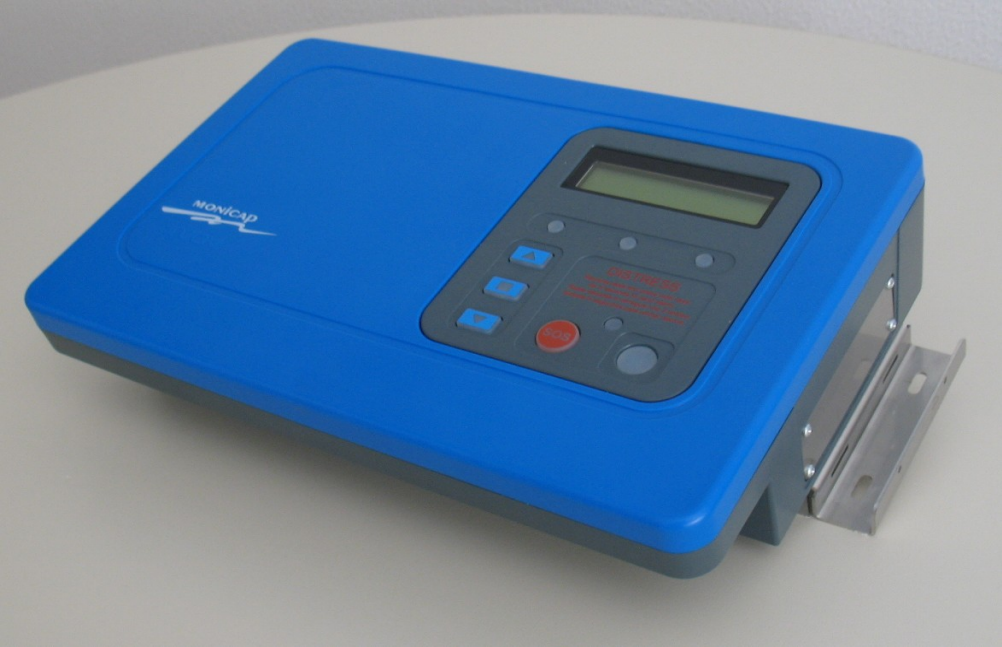
\includegraphics[width=0.8\linewidth]{Chapters/img/equipamento_monicap.png}
\caption{MONICAP Blue Box.}
\label{fig:monicap}
\end{figure}

As MONICAP systems are installed on ships, they can, in real-time, send alerts to the authorities whenever an abnormal change is detected concerning the standard.


\section{Fishing Velocity Patterns} % (fold)
\label{sub:fishing_velocity_patterns}

To know whether a vessel is fishing, we can use its velocity patterns, given that the speed of the vessel differs when it is traveling or when it is fishing. We can verify this fact in the histogram shown in Figure \ref{fig:histogram_vessel2}, corresponding to a vessel velocity.

In Figure \ref{fig:histogram_vessel2}, the histogram allows us to recognize two different velocity patterns, identified by two distinct distributions. They are visible when we graphically represent the velocity's data of each of the vessels. The distribution characterized by lower average speeds corresponds to fishing activity, and the other speed distribution corresponds to the movement of the vessel between the port and the fishing sites \cite{MappingFishing}. \\
So, it is needed to isolate the first distribution's range to be able to classify the upcoming future velocity's as being fishing associated or not.
\begin{figure}[H]
\centering
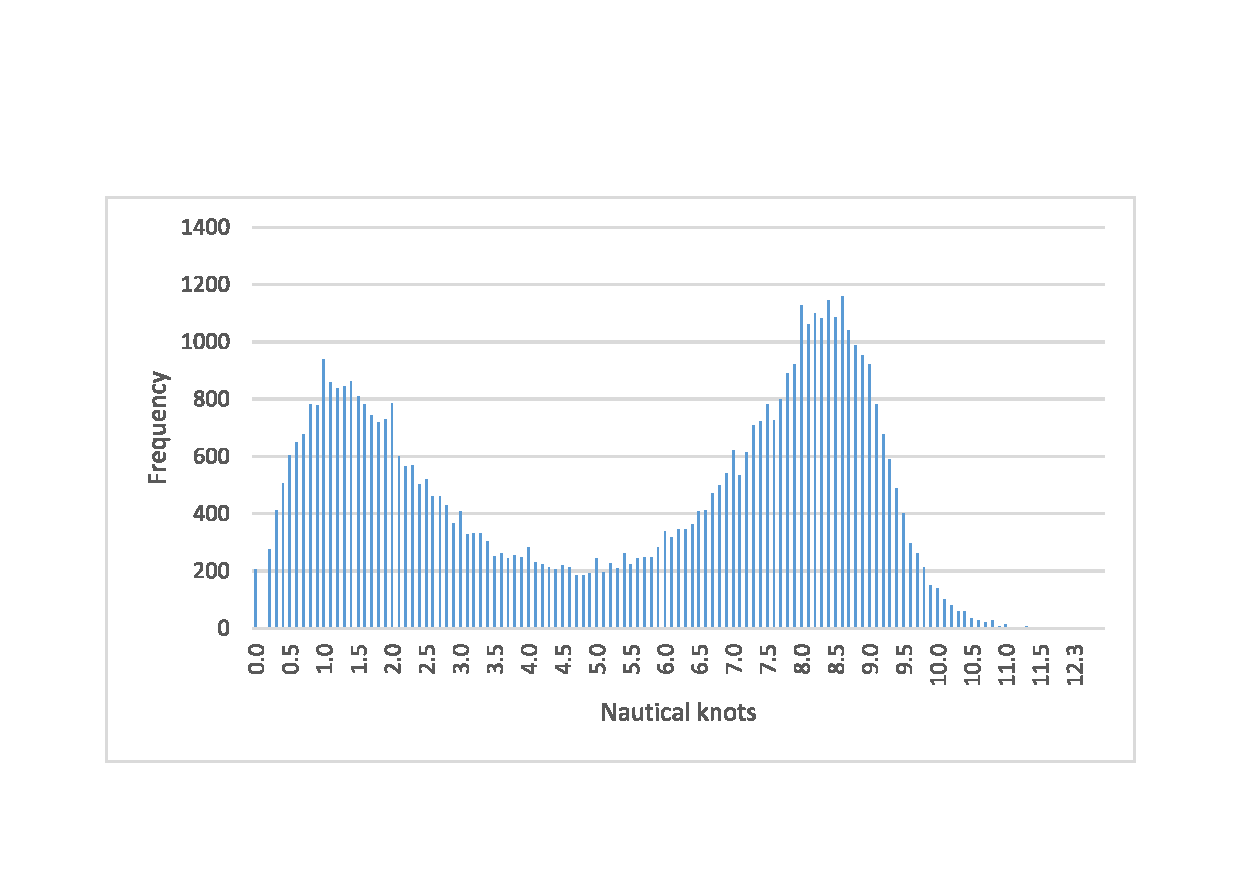
\includegraphics[trim=0 50 0 50, width=0.8\linewidth]{Chapters/img/hist_vessel2.pdf}
\caption{SOG Histogram vessel 2.}
\label{fig:histogram_vessel2}
\end{figure}


For the purpose of isolating the first distribution we considered and analyzed the potential of two different procedures:
\begin{itemize}

\item \textbf{Kernel Density Estimation:} Method explained in Sub Chapter \ref{subsub:kernel_density}.

The implementation used was KernelEstimator from the WEKA library  \cite{WEBSITE:Weka}.

 

\item \textbf{Filter:}
Use a Hill-Climbing algorithm explained in Sub Chapter \ref{subsub:hill_climbing_algorithm}.
With this algorithm, the first maximum is found, and then the algorithm identifies the next minimum.
Then remove all the velocity occurrences that happen to be less than 10 \% of the maximum occurrence and isolating the occurrences that are followed. A clean distribution of the fishery speed for each vessel is derived. With this, the minimum and the maximum values of this distribution are used to classify the new inputs.
\end{itemize}

After the experiment and the study of all these different methods, the chosen procedure can be described in two steps: it starts by using the method based on the \textbf{Filter} to isolate the fishery speed occurrences from the remaining ones. Then ,the Kernel distribution method was applied.
\begin{enumerate}
\item \textbf{Filter:} In the first step, it retrieves all velocity data from the database to create a histogram like it is shown in Figure \ref{fig:app_b_1}.

\begin{figure}
    \centering
    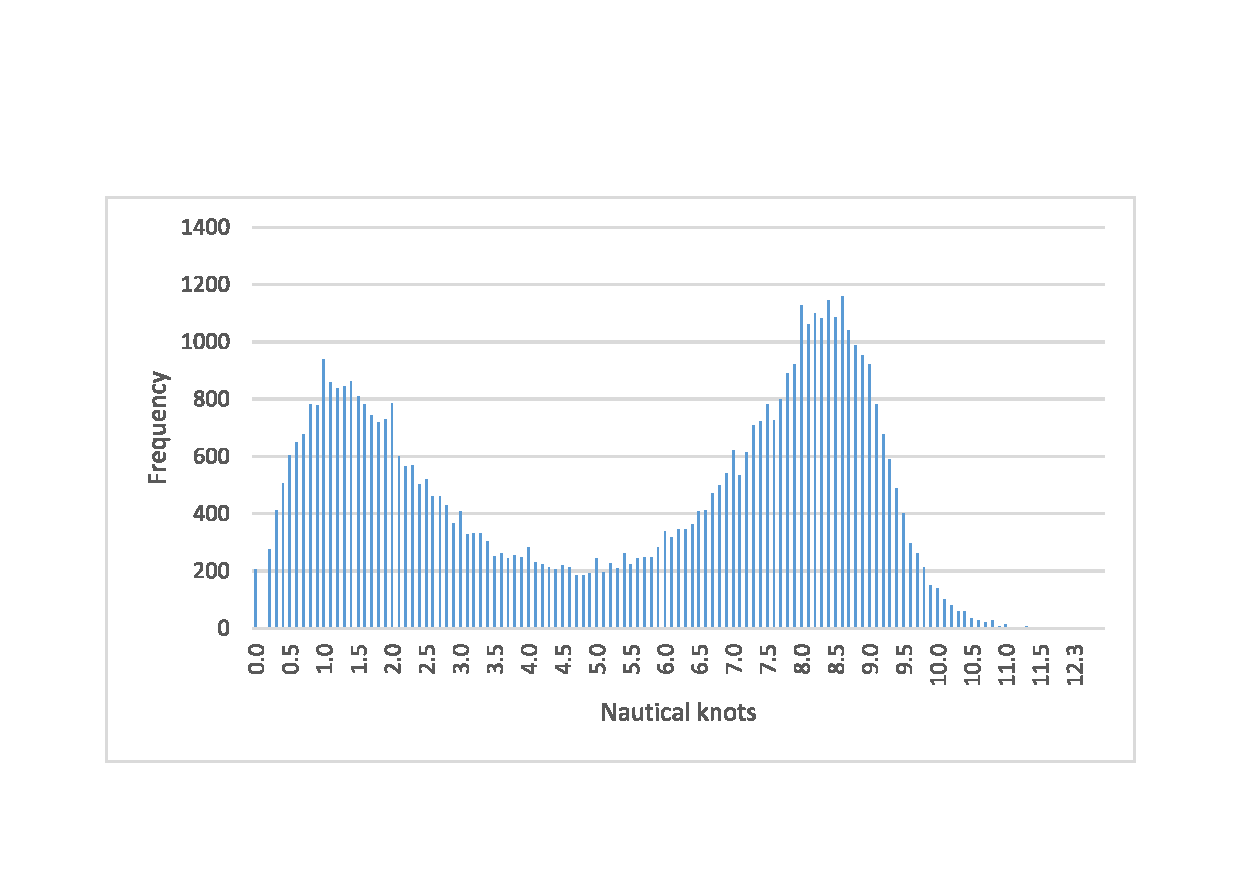
\includegraphics[trim=0 80 0 80,height=0.45\linewidth]{Chapters/img/hist_vessel2.pdf}
    \caption{Velocity histogram in nautical knots}
    \label{fig:app_b_1}
\end{figure}

In the next step, all observations corresponding to zero velocities were removed, because we do not want to consider when the vessel is completely stopped. Then it uses the hill-climbing algorithm to get the minimum and the maximum value of the first distribution. 
The implementation of the hill climbing algorithm used consisted of identifying the maximum, then continuing the search, to determine the distribution limit.
%The implementation used was altered in a way that when the algorithm converges to the maximum, it will continue to find the limit of the distribution.
To obtain this solution, the algorithm searches for the first local maximum that has not have a higher value in the following three points, as shown in Figure \ref{fig:app_b_3}.



\begin{figure}
    \centering
    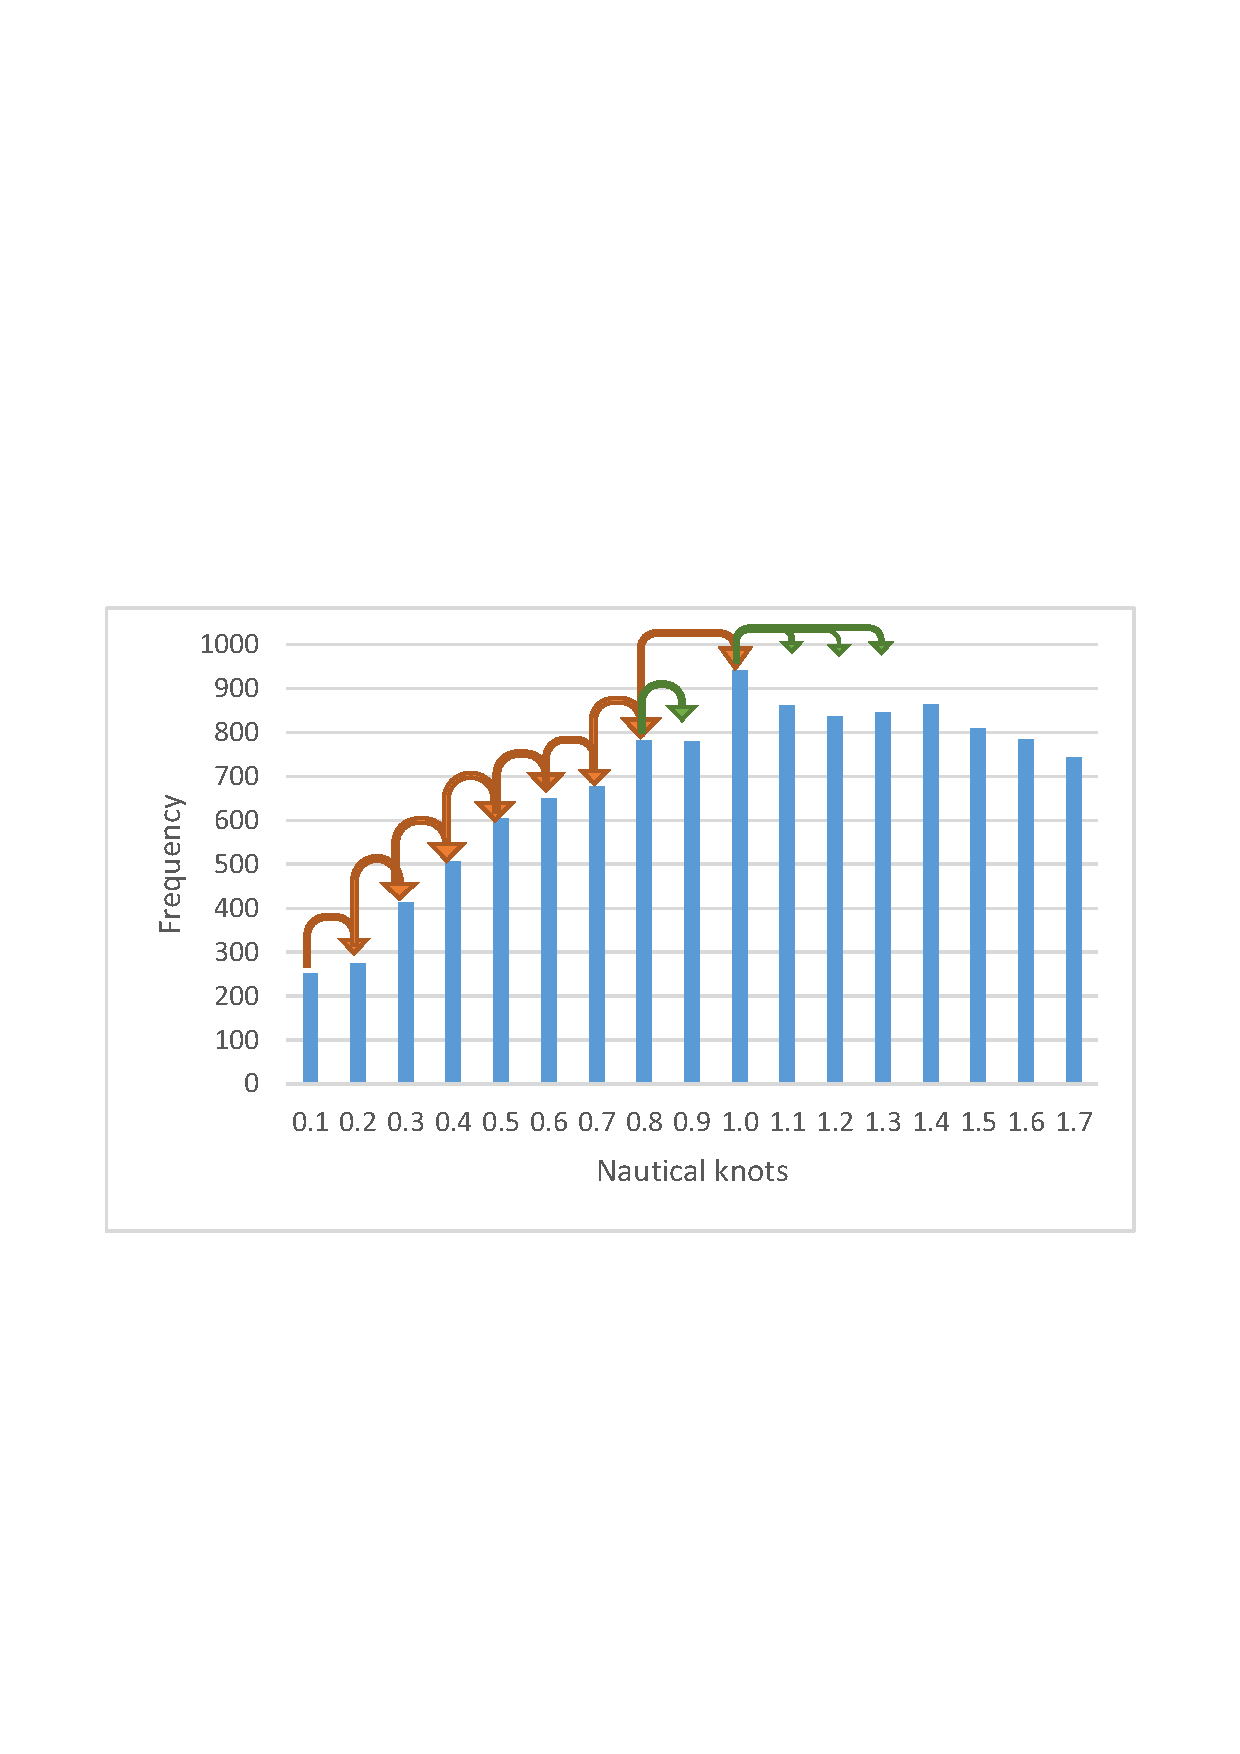
\includegraphics[trim=300 250 300 300,height=0.5\linewidth]{Chapters/img/hc_3.pdf}
    \caption{Hill climbing algorithm step to find maximum}
    \label{fig:app_b_3}
\end{figure}

In this way, we can find the maximum value of the fishing speed range. \\
To find the end of the fishing speed range, the algorithm continues to sweep the histogram until the next three points are not lower than the current point as shown in Figure \ref{fig:app_b_4}.

\begin{figure}
    \centering
    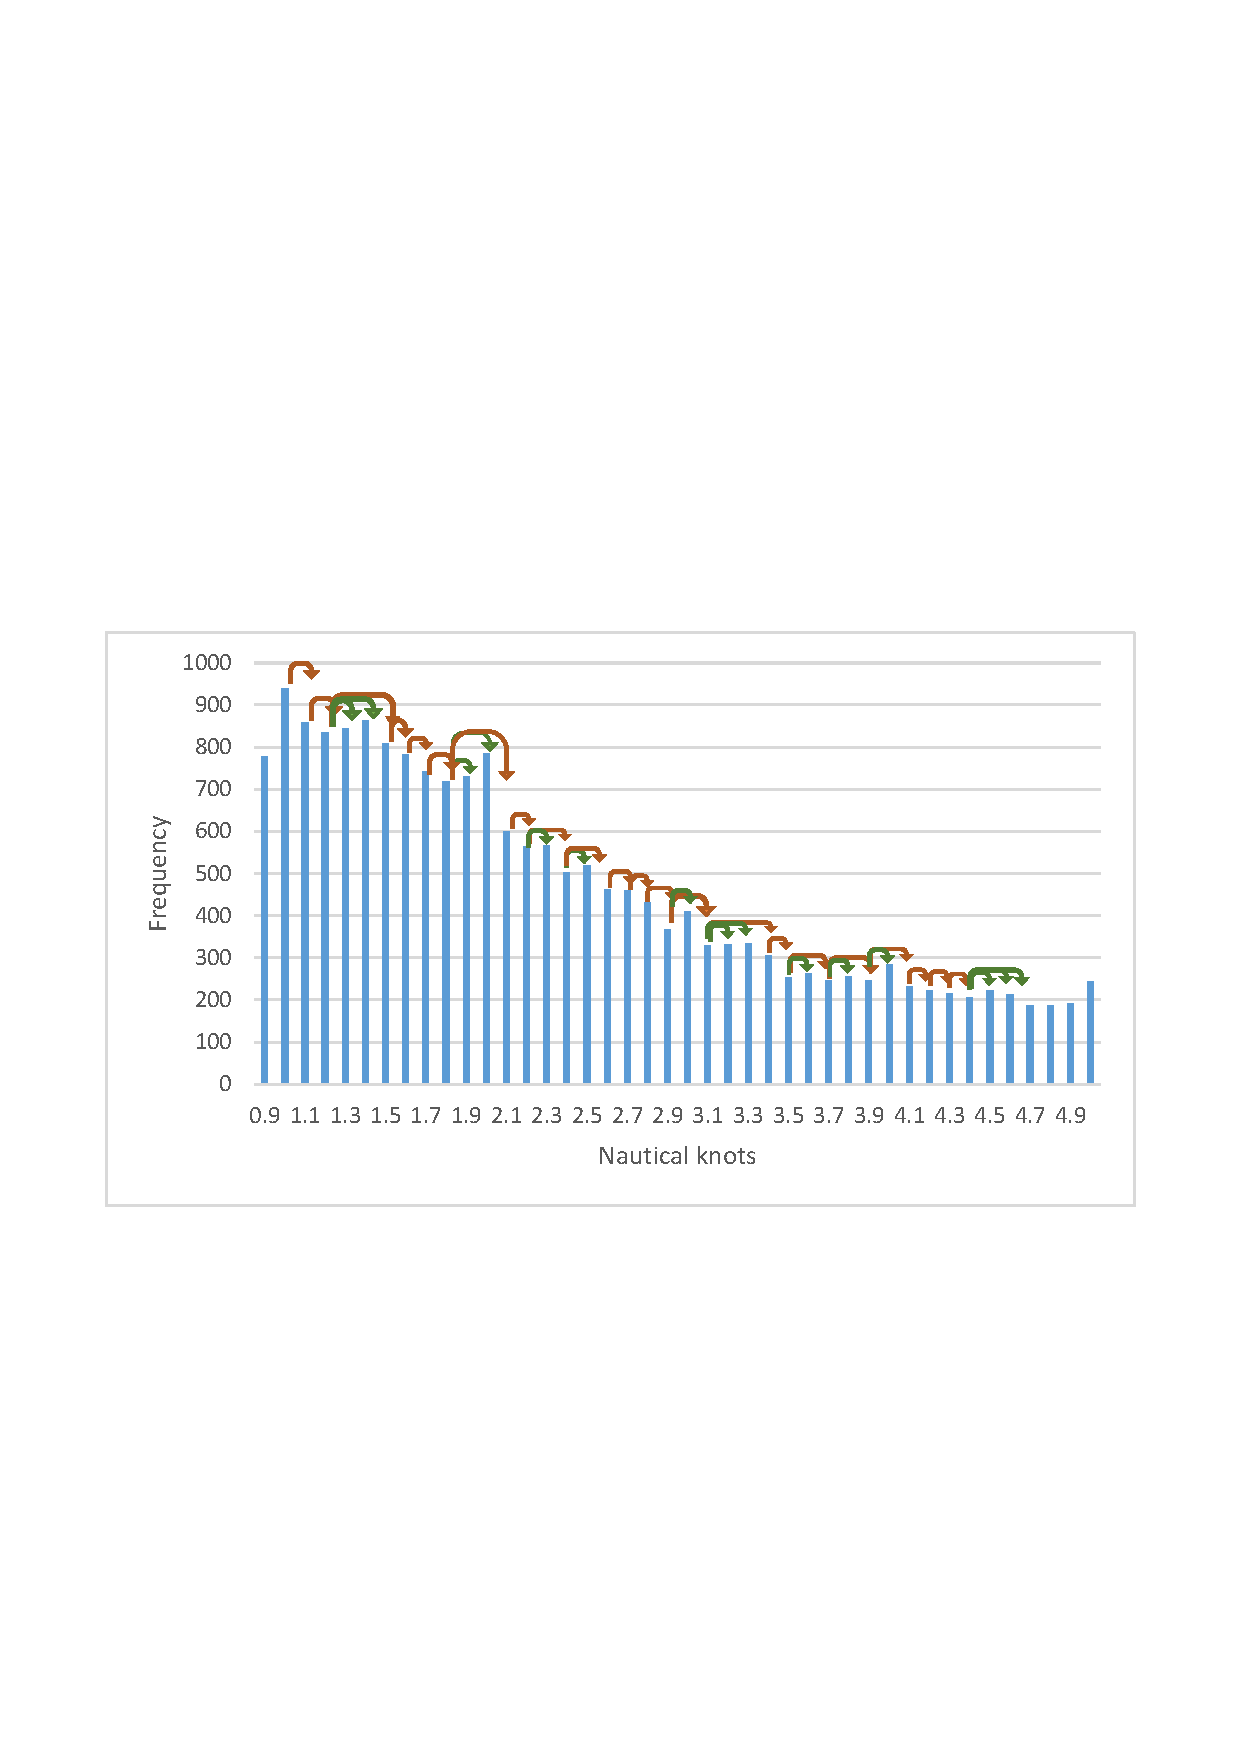
\includegraphics[trim=250 250 250 300,height=0.5\linewidth]{Chapters/img/hc_4.pdf}
    \caption{Hill climbing algorithm step to find minimum}
    \label{fig:app_b_4}
\end{figure}

This way, we can end up with a histogram of the intended distribution, as we can observe in Figure \ref{fig:app_b_5}.


\begin{figure}
    \centering
    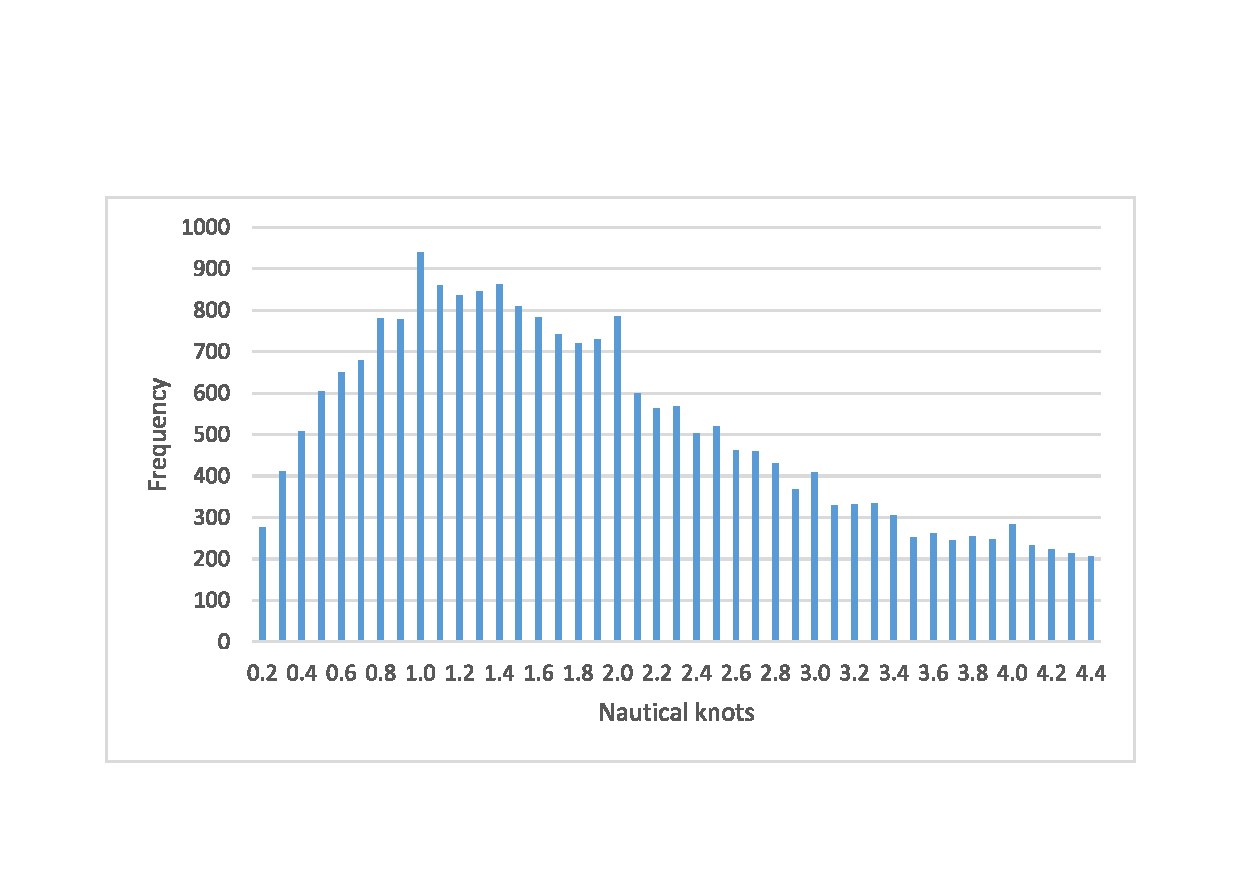
\includegraphics[trim=0 80 0 80,height=0.45\linewidth]{Chapters/img/sog_hill_climbing.pdf}
    \caption{Speed distribution after removing traveling occurrences}
    \label{fig:app_b_5}
\end{figure}

\item \textbf{Kernel method :} It was applied a kernel distribution method in the filtered histogram to have the distribution represented in orange on \ref{fig:app_b_6}. Then, it was created a dictionary with the velocities and the cumulative percentage of velocity. This way, we end up with a representation like the one presented in Figure \ref{fig:app_b_7}. 
Then, a range across quantiles is defined for some probability. Considering this last distribution, a confidence area is defined through a probability. The speeds within this area correspond to fishing activity. Thus, two-speed limits are identified and used to classify the new data.
For the example in Figure \ref{fig:app_b_8}, the output corresponds to the following values: minimum= 0.6, maximum= 3.5.  

\end{enumerate} 

%\newpage
%\begin{lstlisting}
%// Import Weka
%import weka.estimators.KernelEstimator;

%// Create KernelEstimator object with precision as 0.05
%//precision - the precision to which numeric values are given. For example, %if the precision is stated to be 0.1, the values in the interval (0.25,0.35] %are all treated as 0.3.
%KernelEstimator kernel = new KernelEstimator(0.05);

%// Add number of occurrences by velocity
%kernel.addValue(entry.getKey(), entry.getValue());

%// Get velocity keys
%double[] means = kernel.getMeans();

%//for each velocity key, get the probability of having occurrence 
%for (double d : means) {
% 	double prob = kernel.getProbability(d);
%}
%\end{lstlisting}


\begin{figure}[H]
    \centering
    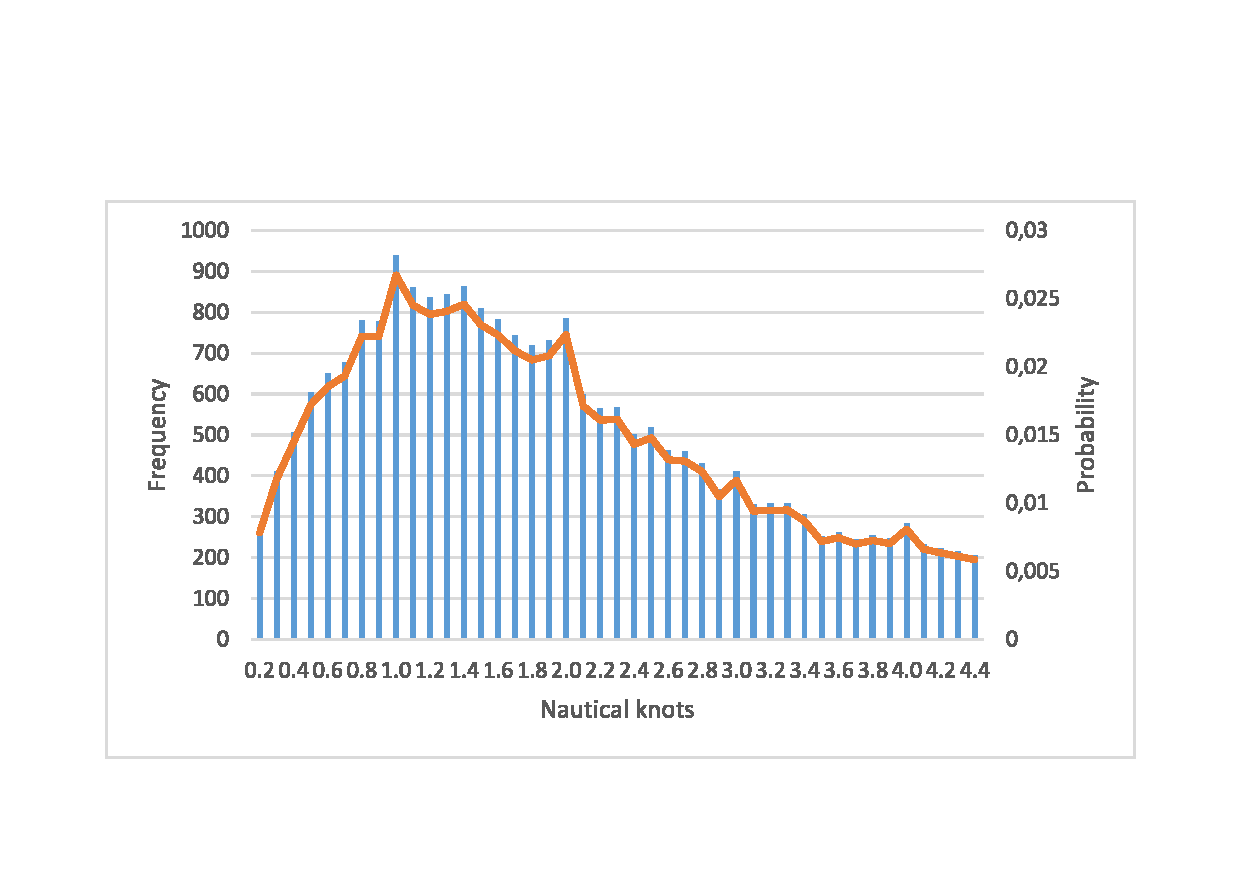
\includegraphics[trim=0 80 0 80,height=0.45\linewidth]{Chapters/img/hist_kernel.pdf}
    \caption{Estimated Kernel Density function}
    \label{fig:app_b_6}
\end{figure}


\begin{figure}[H]
    \centering
    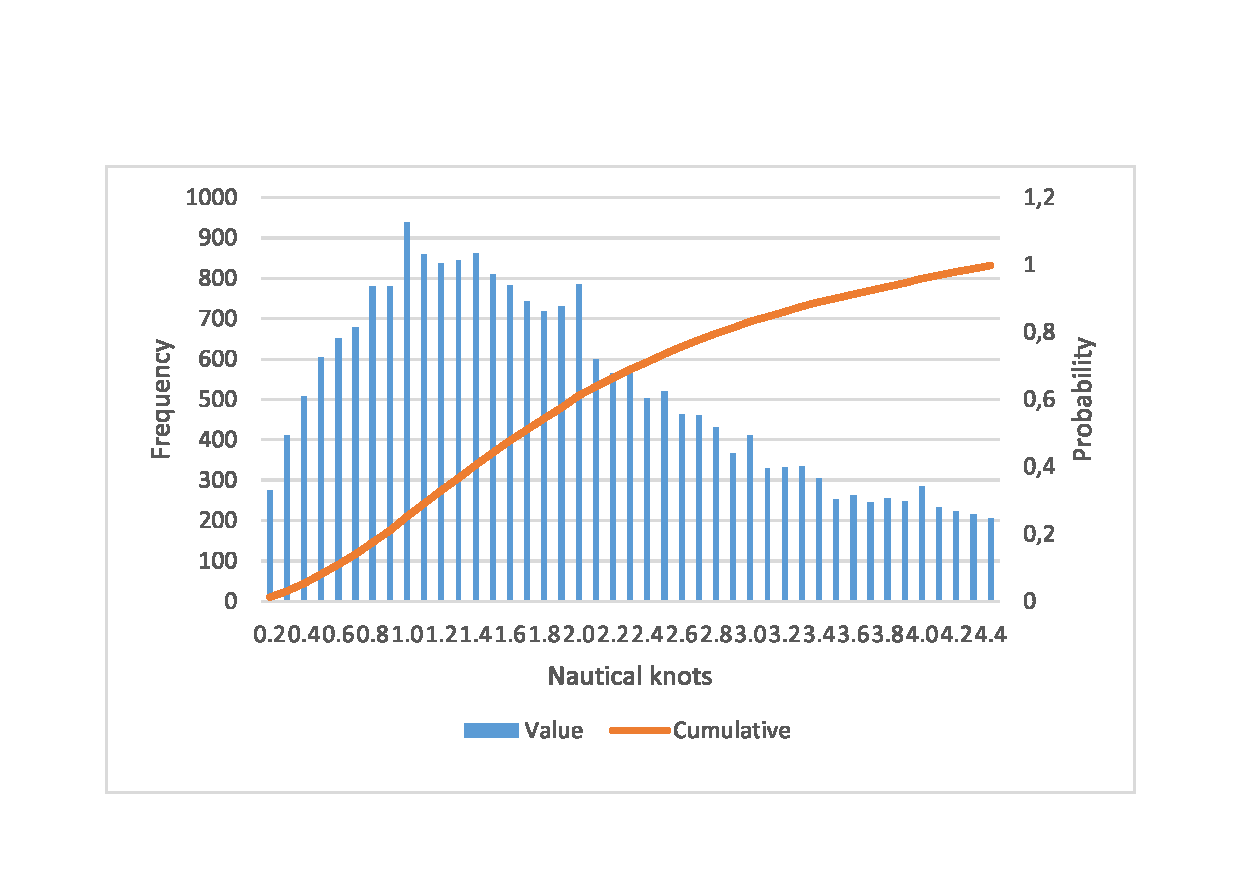
\includegraphics[trim=0 80 0 80,height=0.45\linewidth]{Chapters/img/hist_comulative.pdf}
    \caption{Estimated Cumulative Kernel distribution}
    \label{fig:app_b_7}
\end{figure}


\begin{figure}[H]
    \centering
    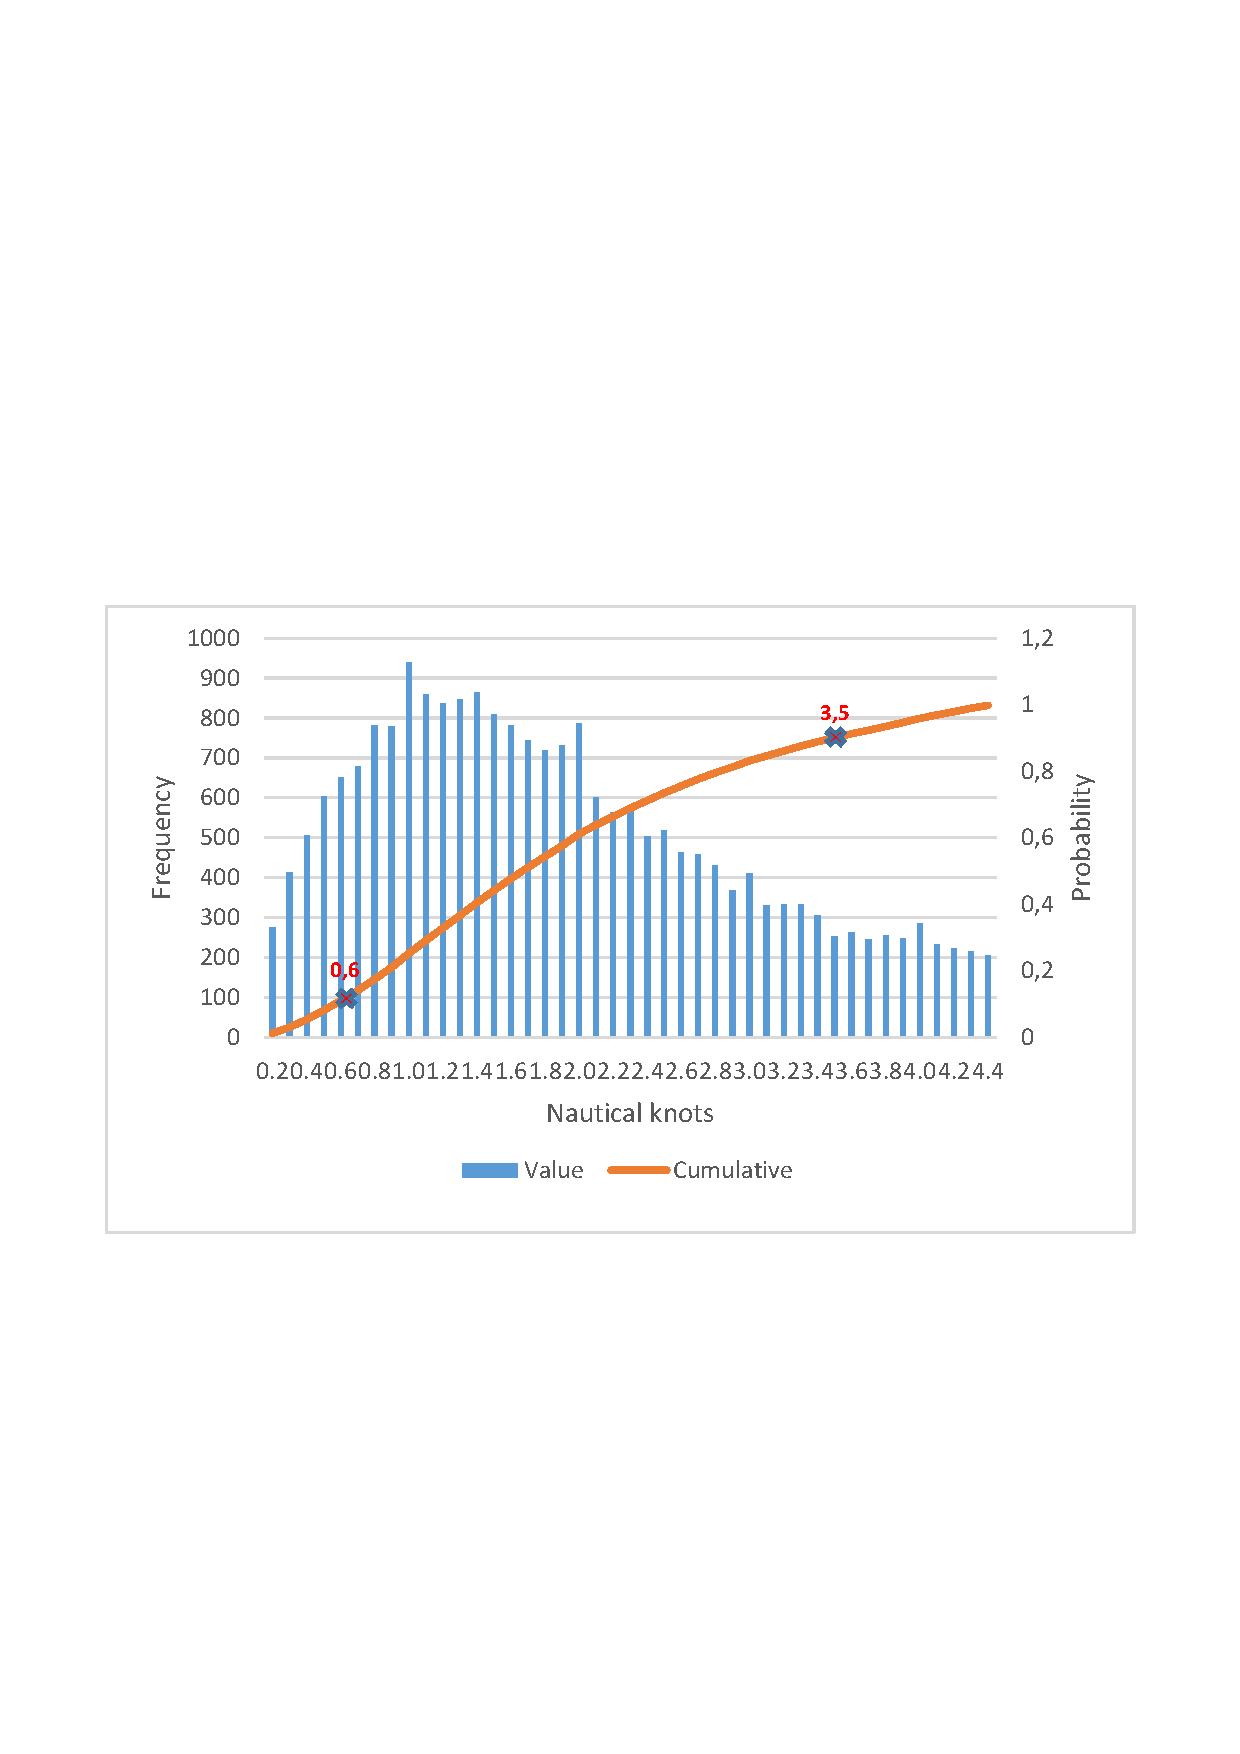
\includegraphics[trim=300 250 300 300,height=0.5\linewidth]{Chapters/img/hc_8.pdf}
    \caption{Set margin and get limits}
    \label{fig:app_b_8}
\end{figure}


Now, we can compare the new data with the established limits. If the new data is within limits, we classify as fishing, and if not, we classify as not fishing.

% section fishing_velocity_patterns (end)


\section{Fishing Spots} % (fold)
\label{sub:fishing_spots}

To discover whether the vessel is fishing in its fishing zone, or in a new location, the history of GPS locations by vessel was used.
Fishing in a new zone may mean that the vessel has changed its type of fishing or is engaging in an activity that is not licensed.


\begin{figure}[]
\centering
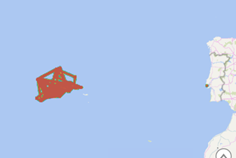
\includegraphics[width=0.8\linewidth]{Chapters/img/gps_vessel2.png}
\caption{Vessel 2 geographic coordinates}
\label{fig:gps_vessel2}
\end{figure}

In Figure \ref{fig:gps_vessel2}, we can see the geographic coordinates points for the vessel 2. Using methods based on clustering, it is possible to identify, by vessel, several areas that are the standard fishing zones of this vessel. When the vessel is outside that standard zone, a flag should occur.

Using the fishing velocity range encountered in the previous point, we get the GPS points of the vessel within that range, so we can work only with the positions where the vessel was fishing. The next step is to use a clustering algorithm to define the fishing areas so that we can compare it with the new GPS points. 

For this purpose, several data mining algorithms were performed in order to choose the best results:

\begin{itemize}
\item \textbf{K-Means:} Method explained in Sub Chapter \ref{sub:kmeans}. The implementation used was SimpleKMeans from WEKA library.


\item \textbf{Density Based Cluster:} Method explained in Sub Chapter \ref{subsub:density_based_c}. The implementation used was MakeDensityBasedClusterer from WEKA library.
 

\item \textbf{DBSCAN:} Method explained in Sub Chapter \ref{subsub:dbscan}. The implementation used was DBSCAN from WEKA library.

\end{itemize}

After some tests, it was decided that Density-Based Cluster is the best approach for this case. It was excluded DBSCAN, because as we can observe in Table \ref{table:mill_per_moodle}, this model needs much processing power to estimate the clusters. These values were retrieved using a computer with an Intel i5 (2.5 GHz) processor and 8 GB of RAM. Considering that the Blue Box has a lot less processing power, it was decided that this model is not a good solution for this problem.
\\

\begin {table}[]
\caption {Time of processing in miliseconds per model}
\begin{center}
\begin{tabular}{c|c|c|c}
& \textbf{K-Means} & \textbf{Density Based Cluster} & \textbf{DBSCAN} \\
\hline
Initializing & 862 & 923 & 25848 \\

New data & 25 & 45 & 35 
\label{table:mill_per_moodle}
\end{tabular}
\end{center}
\end {table}

The choice between K-Means and Density-Based Cluster algorithms was based on the fact that Density-Based Cluster represents a great advantage because it estimates the probability of the new geographic coordinates belonging to a cluster-based in the specific cluster probabilistic distribution. This way, the user can choose the most suitable configuration. The resulting clusters themselves are equal when K-Means or Density-Based Cluster were applied since Density-Based Cluster uses K-Means to define the centroids, so they only differ by adding a layer to define the area of density per cluster.
\\


%\begin{lstlisting}
%// Import Weka
%import weka.clusterers.MakeDensityBasedClusterer;
%import weka.core.Instances;
%import weka.core.Instance;
%import weka.core.DenseInstance;
%
%// Create MakeDensityBasedClusterer object
%MakeDensityBasedClusterer density = new MakeDensityBasedClusterer();
%// Set number of clusters
%this.density.setNumClusters(nClusters);
%//Get GPS vessel data
%Instances data = dbAcess.GetArea(this.limits);
%//Create clusters
%this.density.buildClusterer(data); 
%		    	     
%//Create object to get distributions 
%//point is double[] {latitude, longitude}
%Instance test = new DenseInstance(2, point); 
%
%//Returns the clusters probability distribution for an instance.
%double[] distibutionI = this.density.distributionForInstance(test);
%
%//Computes the density for a given instance.  Bigger value, farthest from centroid
%this.density.logDensityForInstance(test) 
%
%\end{lstlisting}


One of the important steps when performing the cluster analysis is the determination of the number groups. To fix the number of groups we can use some indicators such as: coefficient of Silhouette as seen in Sub Chapter \ref{subsub:silhouette}, the coefficient of Davies Bouldin, the coefficient of Calinski Harabasz and the Elbow method as seen in Sub Chapter \ref{subsub:elbow_method}. 


In Figure \ref{fig:elbow_method} is presented the value of the within sum of squares as function of the number of clusters, using the geographic coordinates data for vessel 2. As we can observe, six clusters seems to be a good number as the error is not decreasing much as the number of clusters increases. 


\begin{figure}[]
\centering
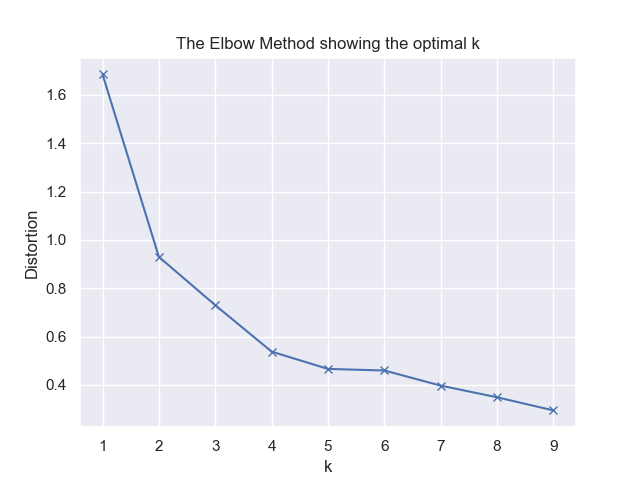
\includegraphics[width=0.8\linewidth]{Chapters/img/elbow_method.png}
\caption{Sum of squared error as function of the number of clusters}
\label{fig:elbow_method}
\end{figure}


The average value of the Silhouette coefficient for vessel 2 is as described in Table \ref{table:vessel2_silhouette} with nine and six having good values.

\begin {table}[h]
\caption {The average value of the Silhouette coefficient for vessel 2}
\begin{center}
\begin{tabular}{c|c}
\textbf{Number of clusters} & \textbf{Average silhouette coefficient}  \\
\hline
2 & 0.5933  \\
3 & 0.5950  \\
4 & 0.5510  \\
5 & 0.6233  \\
6 & 0.6635  \\
7 & 0.6319  \\
8 & 0.6514  \\
9 & 0.6907  
\label{table:vessel2_silhouette}
\end{tabular}
\end{center}
\end {table}


Considering the two methods I chose six as the number of clusters for the vessel 2.

% section fishing_spots (end)



\section{SFA Library} % (fold)
\label{sub:sfa_library}

It was created a software application called SFALib for (Standalone Fishery Analysis Library) that can be find in a online repository \cite{sfagithub}. In this application, were developed the solutions described in this chapter to help with the elaboration and tests for this project. For a market solution, this library could be used by the main application of a Blue Box, to send alerts to support decision making or to simply classify each VMS data entry into two categories:
\begin{enumerate}
\item Is fishing (yes/no).
\item Is fishing in a new area (yes/no).
\end{enumerate}



\subsection{Functionality} % (fold)
\label{sub:functionality}

This application allows to:
\begin{itemize}
\item Test new data \\ Send and receive VMS data, if it is considered to be fishing and if it is in a new area.
\item Test new velocity \\ Send sog data and receive true if it is considered to be fishing.
\item Test new location \\ Send GPS data and receive true it is in a new area.
\item Restart models \\ Request to create new models. It can be used if the objective is running for a long time and want to renew models with new data. 
\item Get limits \\ Request the velocity limits. Receive a tuple with two doubles (item1 = low-speed limit, item2 = high-speed limit). It can be used for analysis like described in Chapter 4.
\end{itemize}

To make this possible, it is necessary to configure the data access layer to get the VMS data from the local data repository. The data repository used in this work to save and access VMS data was a database but could be other type like text files. The type of data repository used by MONICAP was not revealed to me.
Currently, the application supports connection to SQL Server \cite{WEBSITE:SqlServer} and PostgreSQL \cite{WEBSITE:Postgresql}.


% subsection functionality (end)


\subsection{Architecture and Implementation} % (fold)
\label{sub:architecturee_implementation}
To develop the software, it was decided to use Java 8 \cite{WEBSITE:OraJava8} because it is a powerful, full object-oriented, and cross-platform programming language. MONICAP uses Linux, so using a JRE (Java Runtime Environment) application is a good choice.
The architecture is depicted in Figure \ref{fig:SFALib_Prof}. In this architecture, it is possible to distinguish three main modules: One that is the core of the SFALib, create the modules and use them. Another one is WEKA \cite{WEBSITE:Weka} that creates the cluster modules for locations and implements the Kernel density estimation  for velocity. The last one is the data access layer that is responsible for getting the VMS data from the local repository so SFALib can create the modules.


\begin{figure}[]
\centering
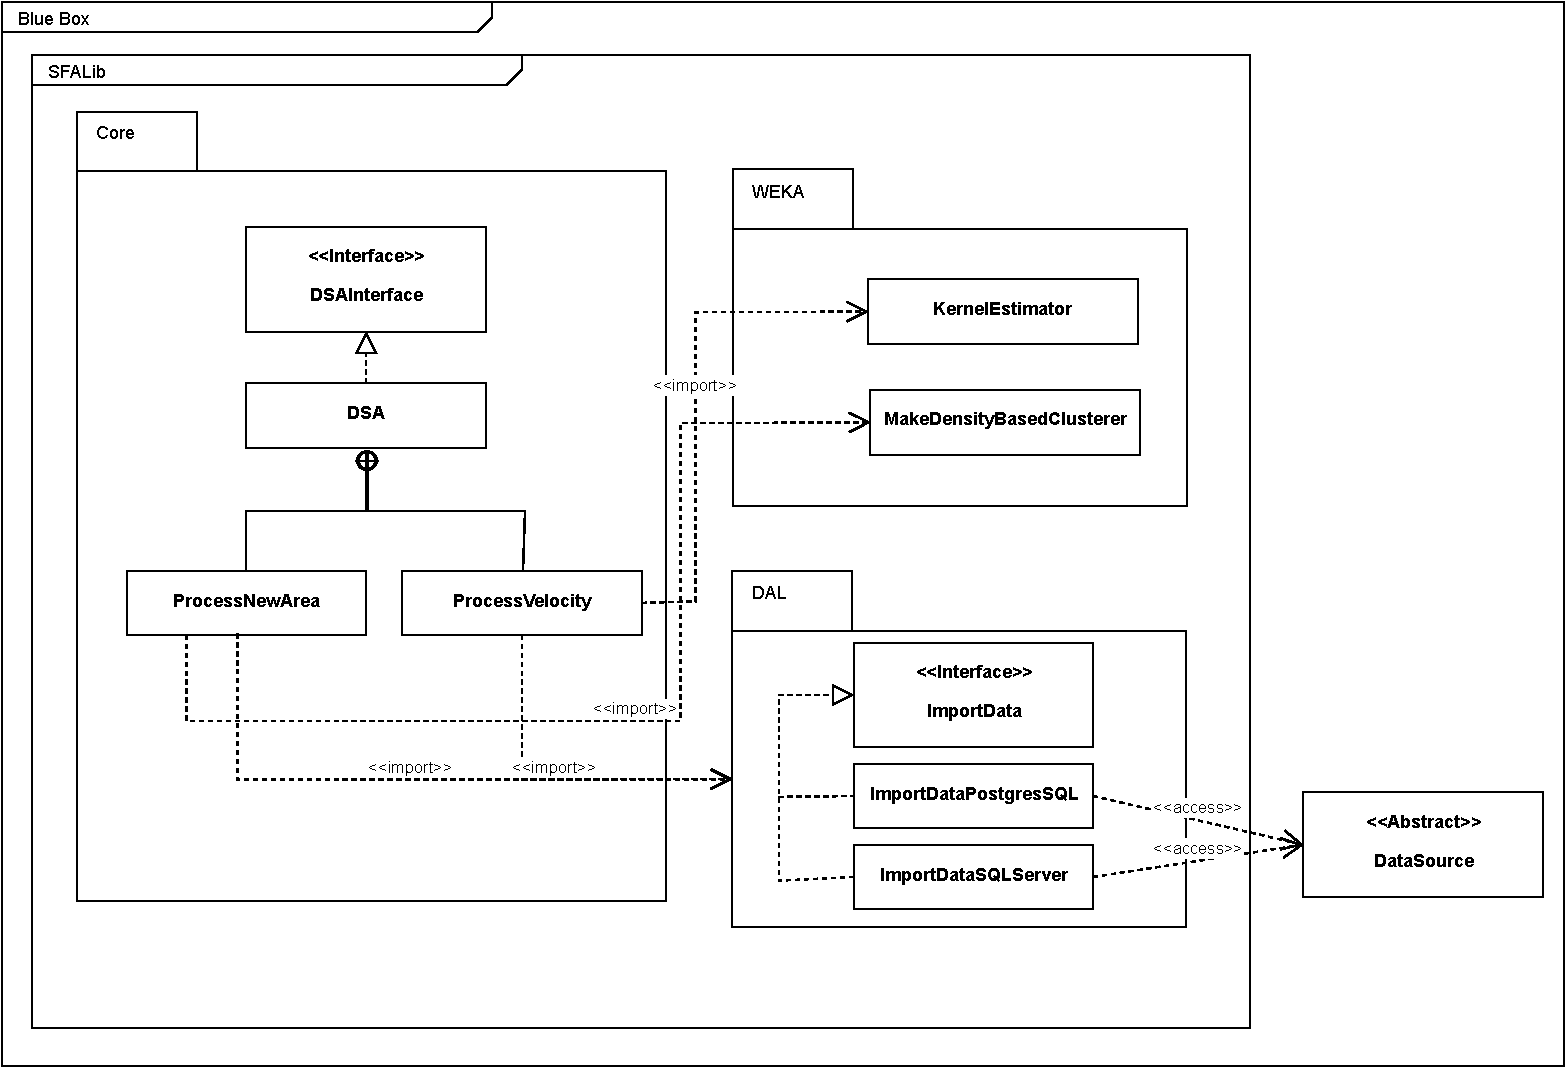
\includegraphics[width=1.0\linewidth]{Chapters/img/SFALib_Prof.pdf}
\caption{Representation of the SFALib architecture.}
\label{fig:SFALib_Prof}
\end{figure}



\textbf{Core module} \\The core module is responsible for initializing the models and using them the way described in this chapter. The procedure starts with the creation of an instance, called  "ProcessVelocity", whose objective is to use the historical speed data of the ship to classify whether or not it is fishing. After that, is created another instance called, "ProcessNewArea", whose objective is to identify if a new data (geographic coordinates) is or is not in a usual fishing location for that vessel, using for that purpose the history of the vessel's GPS locations.

\textbf{WEKA module} \\WEKA is a collection of machine learning algorithms for data mining tasks. It contains tools for data preparation, classification, regression, clustering, association rules mining, and visualization. In this application, WEKA is used as a tool to create the modules.

\textbf{DAL module} \\The data access module was implemented in a way not only to get data but also to filter data in the database engine. Filtering data (where) is optimized on the database engine, and so we gain some performance.




The application starts by initializing two objects:
\begin{enumerate}
\item ProcessVelocity: This object is responsible for doing the process explained in section 4.2 of this document. It will request to the static class ImportData to retrieve all SOG (Speed Over Ground) data from the database. Then, the process will end with the limits (minimum speed of fishing and the maximum speed of fishing).
\item ProcessNewArea: This object is responsible for doing the process explained in section 4.3 of this document. This object is only initialized after ProcessVelocity because it needs the velocity fishing limits necessary to create the clusters of the fishing areas. With these limits, the object requests to the ImportData instance to obtain the latitude and longitude values where the vessel was in between the velocity limits. With this, the object ends up with the clusters of the fishing areas.
\end{enumerate}


% subsection architecturee_implementation (end)

\subsection{Deployment} % (fold)
\label{sub:deployment}

We start by initializing SFALib with the doubles \emph{limitVelocity} and \emph{limitArea}. These doubles range between 0 and 1:
\begin{itemize}
\item limitVelocity: used to get the maximum and minimum speed by reducing the speed range. This limit will reduce the maximum speed and increase the minimum speed by setting the maximum velocity as the velocity that as (1-limit) percentage of the cumulative kernel distribution and the minimum velocity as the velocity that has a (limit) percentage of the cumulative kernel distribution.
\item limitArea: used to compare with the probability to belong in a cluster given to the new points. If the limit is smaller than the given probability, then the vessel is classified as fishing in a new area.
\end{itemize}
These limits could be defined by the user. This possibility allows to configure the application according to the preference in obtaining more false positive or false negative classifications.
A false positive (type I error) is when the classifier rejects a true hypothesis.
A false negative (type II error) is when the classifier accepts a false hypothesis.

After the SFALib is ready, we need to send a new velocity data and GPS coordinates to receive an object with an "isFishing" as true if the vessel is fishing. "isNewArea" as true if the vessel is in an area that is not a normal fishing area and it's in a fishing velocity.

The methods that can be used are:
\begin{itemize}
\item newData: method that receives VMS data and returns isFishing(boolean) and isNewArea(boolean).
\item isFishing: method with SOG (double) as input and a boolean as output with, True = is fishing, False = not fishing.
\item isNewArea: method with geographic coordinates (double longitude, double latitude) as input and a boolean as output with, True = is fishing in a new area, False = not fishing in a new area.
\item restart: this method restarts the models. It can be used to create models with new data.
\item GetLimit: the method used to get SOG limits used by the SFALib to classify velocity. Returns SOG limits as doubles.
\end{itemize}
% subsection usage (end)

% section SFA_library (end)
% chapter blue_box (end)





